\documentclass[a4paper,11pt,french]{book}
\usepackage[utf8]{inputenc}

\usepackage[T1]{fontenc}
\usepackage[francais]{babel} 
\usepackage[top=2cm, bottom=2cm, left=2cm, right=2cm, includeheadfoot]{geometry} %pour les marges
\usepackage{lmodern}
\usepackage{pict2e}
\usepackage{tikz}	
%\usepackage{tikz-uml}
\usepackage{fancyhdr} % Required for custom headers
\usepackage{lastpage} % Required to determine the last page for the footer
\usepackage{extramarks} % Required for headers and footers
\usepackage{graphicx} % Required to insert images
\usepackage{tabularx, longtable}
\usepackage{color, colortbl}
\usepackage{lscape}
%\usepackage[hidelinks]{hyperref}
\usepackage{longtable}
\usepackage{multirow}
\usepackage{rotating}
%\usepackage{pgfgantt}
\usepackage{gensymb}
\usepackage[toc,page]{appendix} 
\usepackage{pgfplots}
\usepackage{eurosym}
\usepackage{rotating}
\usepackage{array}
\usepgflibrary{arrows} % for pgf-umlsd

\usetikzlibrary{trees,shapes.geometric,arrows,decorations.pathmorphing,backgrounds,fit,positioning,shapes.symbols,chains	}
 \tikzset{
    %Define standard arrow tip
    >=stealth',
    %Define style for boxes
    punkt/.style={
           rectangle, dashed,
           rounded corners,
           draw=black, very thin,
           minimum height=2em,
           minimum width = 2cm,
           text centered},
    square/.style={
           rectangle,
           draw=black, thick,
           minimum height=.5cm,
           minimum width = 1cm,
           text centered},
    data/.style={
           rectangle,
           draw=black, thick,
           minimum height= 2cm,
           minimum width = 2cm,
           text centered},
    % Define arrow style
    pil/.style={
           ->,
           thick,
           shorten <=1pt,
           shorten >=1pt,},
    asym/.style={
           <->,
           thin,
           shorten <=1pt,
           shorten >=1pt,
           red!100},
    sym/.style={
           <->,
           thin,
           shorten <=1pt,
           shorten >=1pt,
           blue!100}
}


%\usetikzlibrary{trees,shapes.geometric,arrows,decorations.pathmorphing,backgrounds,fit,positioning,shapes.symbols,chains	}

\linespread{1.1} % Line spacing

% Set up the header and footer
\pagestyle{fancy}
\lhead{\textbf{\hmwkClass -- \hmwkSubject \\ \hmwkTitle \\ \hmwkDocName}} % Top left header
\rhead{
\includegraphics[width=10em]{logo_univ.png}}
\lfoot{\lastxmark} % Bottom left footer
\cfoot{} % Bottom center footer
\rfoot{Page\ \thepage\ } % Bottom right footer
\renewcommand\headrulewidth{0.4pt} % Size of the header rule
\renewcommand\footrulewidth{0.4pt} % Size of the footer rule

\setlength{\headheight}{40pt}

\newcommand{\hmwkTitle}{Chat sécurisé} % Assignment title
\newcommand{\hmwkClass}{Master 1 SSI } % Course/class
\newcommand{\hmwkAuthorName}{Charles Ango, Ismael Kabore,  Julien Legras, Yves Nouafo, Jean-Baptiste Souchal} % Your name
\newcommand{\hmwkSubject}{Conduite de projet} % Subject
\newcommand{\hmwkDocName}{Rapport de projet} % Document name

\newcommand{\version}{1.2} % Document version
\newcommand{\docDate}{24 mai 2013} % Document date
\newcommand{\checked}{Magali Bardet} % Checker name
\newcommand{\approved}{} % Approver name

\definecolor{gris}{rgb}{0.95, 0.95, 0.95}

\title{
\vspace{2in}
\textmd{\textbf{\hmwkClass :\ \hmwkTitle}}\\
\normalsize\vspace{0.1in}\small{Due\ on\ \hmwkDueDate}\\
\vspace{0.1in}\large{\textit{\hmwkClassInstructor\ \hmwkClassTime}}
\vspace{3in}
}

\author{\hmwkAuthorName}
\date{} % Insert date here if you want it to appear below your name

\makeatletter
\def\chapter{\if@openright\cleardoublepage\else\clearpage\fi
  \global\@topnum\z@
  \@afterindentfalse
  \secdef\@chapter\@schapter}
\makeatother


\begin{document}
\pagestyle{empty}

\vspace*{1cm}
\begin{center}

\includegraphics[width=20em]{logo_univ.png}
\end{center}
\vspace*{2cm}
\begin{center}\textbf{\huge{Master 1 Sécurité des systèmes informatiques}}\end{center}
\vspace*{1cm}
\begin{center}
\textbf{\Huge{\hmwkDocName}: \hmwkTitle}
\end{center}

\vspace*{3cm}
	

\fcolorbox{black}{gris}{
\begin{minipage}{15cm}
\begin{tabularx}{10cm}{lXp{8cm}}
	& & \\
	\bfseries{Rédigé par} & & \hmwkAuthorName \\
	& & \\
	\bfseries{À l'attention de} & & \checked \\
	& & \\
	\bfseries{Date de rendu} & & \docDate\\
	& & \\
\end{tabularx}
\end{minipage}
}

\newpage


%%%%%%%%%%%%%%%%%%%%%%%%%%%%%%%%%%%%%%%%%%%%
% Introduction
% JB
%%%%%%%%%%%%%%%%%%%%%%%%%%%%%%%%%%%%%%%%%%%%
\frontmatter
\pagestyle{fancy}
\large
\chapter{Introduction}

Les outils de messagerie instantanée sont de nos jours largement utilisés par les particuliers et entreprises. Ces communications donnent 
parfois lieu à des échanges de données confidentielles or, la sécurité des données et l'authentification des utilisateurs n'y est géneralement pas assurée. Il est donc important 
d'avoir à disposition des outils permettant d'assurer la confidentialité d'une 
communication. C'est donc dans le cadre de notre projet annuel de première année 
de master en sécurité des systèmes d'information que nous avons étudier les protocoles cryptographiques permettant a plusieurs utilisateurs de s'authentifier et de communiquer de manière securisée a travers un
outil de messagerie instantanée permettant la confidentialité et l'intégrité 
des données échangées.

La couche de sécurité mis en place sur un outil de 
messageris instantanée va permettre de pouvoir dialoguer avec des utilisateurs 
authentifiés dont l'identité est connue, d'avoir la certitude de l'intégrité des 
messages reçus, c'est à dire que le message n'a pas été modifié entre deux 
interlocuteurs puis une confidentialité assurée des contenus échangés grâce à 
des outils cryptographique forts mis en place empêchant toute lisibilité des 
données transitant entre utilisateurs.

Dans un premier temps nous allons faire une présentation plus détaillé du sujet 
en analysant les besoins du client puis nous présenterons les solutions proposées afin 
d'y répondre. Nous détaillerons ensuite les résultats obtenus après 
l'implémentation des solutions proposées en amont et leurs pertinences par rapport aux besoins du client.
Finalement un manuel d'utilisation viendra compléter ce rapport afin d'assurer une 
bonne prise en main de l'outil de messagerie instantanée par le client.

%La table des matières
\tableofcontents



\newpage
\mainmatter
%%%%%%%%%%%%%%%%%%%%%%%%%%%%%%%%%%%%%%%%%%%%
% PRÉSENTATION DU PROJET 
% Yves & Julien
%%%%%%%%%%%%%%%%%%%%%%%%%%%%%%%%%%%%%%%%%%%%
\chapter{Présentation du projet}
Dans le cadre de notre projet, il nous à été demandé de réaliser un chat sécurisé. Pour le mener à bien, le travail à été découpé en deux grandes phases qui sont l'analyse des besoins du client et les solutions proposées.

\section{Besoins du client}
Les besoins du logiciel sont les points indispensables, nécessaires et imposés par le client. Ce sont ces exigences qui détermineront les fonctionnalités du logiciel. Dans notre sujet, on le résume de la manière suivante:\\ 

\textbf{\'Etudier les protocoles cryptographiques permettant à plusieurs utilisateurs de s’authentifier et de communiquer de manière s'écurisée à travers un outil de messagerie instantanée.}\\

\'A l'a fin du développement, l'outil de messagerie instantanée devra répondre aux besoins de la garantie que les messages soient échangés entre utilisateurs, de la preuve de la mise en place du système de sécrurité ainsi que les protocoles déployés pour parvenir à la fin du développement.

\section{Solutions proposées}
\`A l'issue de l'analyse des besoins du client, il a été convenu de traiter sa demande en décomposant la réalisation du logiciel en trois phases de développement.
\begin{itemize}\item \textbf{Phase 1:} Mise en place du système de bavardage modèle client-serveur;\item \textbf{Phase 2:} Installation d'une PKI (infrastructure de clés publiques);\item \textbf{Phase 3:} Mise en place d'une couche sécurisée pour permettre une communication chiffrée.\end{itemize}
\vspace{.5cm}

\subsection{Structure du logiciel}
Le logiciel est conçu et pensé de manière modulable de tel sorte que chaque partie puisse \^etre utilisée de manière indépendante. Son architecture se présente ainsi:\\

\begin{center}
\begin{tikzpicture}[node distance=-.01cm,font=\tiny,scale=1.8,every node/.style={transform shape}]
		\node[square, text width=1.5cm, fill=white!100] (appclient) at (0,0) {Application client};
		\node[square, text width=2cm, fill=white!100] (modclientsec) at (2.5,0) {Module client sécurisé};
		\begin{pgfonlayer}{background} 
		\node[punkt, fit=(appclient)(modclientsec), fill=blue!20] (groupclient) {};
		\end{pgfonlayer}
		
		\node[square, text width=1cm, fill=white!100] (PKI) at (1.4,-1.5) {PKI};
		\node[square, text width=1cm, fill=white!100] (serveur) at (0,-2.5) {Serveur};
		\node[square, text width=1.5cm, fill=white!100] (serveurs) at (2.5,-2.5) {Serveur sécurisé};
		\begin{pgfonlayer}{background} 
		\node[punkt, fit=(PKI)(serveur)(serveurs), fill=green!20] (groupserveur) {};
		\end{pgfonlayer}

		\node[text width=.7cm] (imgbd1) at (0,-4) {
\includegraphics[height=3em]{computer-database.png}};
		\node[square, text width=.5cm, below=of imgbd1, fill=white!100] (bd1){BDD};
		\node[text width=.7cm] (imgfichiers) at (1.4,-4) {
\includegraphics[height=3em]{computer-database.png}};
		\node[square, text width=.7cm, below=of imgfichiers, fill=white!100] (fichiers){BDD};
		\node[text width=.7cm] (imgbd2) at (2.8,-4) {
\includegraphics[height=3em]{computer-database.png}};
		\node[square, text width=.5cm, below=of imgbd2, fill=white!100] (bd2){BDD};

		\begin{pgfonlayer}{background} 
		\node[punkt, fit=(imgbd1) (bd1) (imgbd2) (bd2) (imgfichiers) (fichiers), fill=orange!20] (stock) {};
		\end{pgfonlayer}


		\draw (appclient.east) edge[<->] (modclientsec.west);
		\draw (appclient.south) edge[<->] (serveur.north);
		\draw (modclientsec.south west) edge[<->] (PKI.north);
		\draw (modclientsec.south) edge[<->] (serveurs.north);
		
		\draw (serveur.south) edge[<->] (imgbd1.north);
		\draw (serveurs.south) edge[<->] (imgbd2.north);
		\draw (PKI.south) edge[<->] (imgfichiers.north);
		\draw (PKI.south east) edge[<->] (serveurs.north);
		
		\draw (PKI.west) edge[->, loop left = 90] (PKI.west);

		\end{tikzpicture}
		\end{center} 
		\vspace{.3cm}
		
Sur le schéma précendent on voit bien la séparation de la partie logicielle de la partie sécuritée, mais aussi les différentes ccouches qui interviennent dans le développement du logicielle. Ces couches sont la partie logicielle, la partie réseaux et la partie base de données.\\

La partie logicielle met en place le coté client de l'application. Elle comporte deux modules qui sont l'application cliente et le module client sécurisé. L'application cliente permet à l'utilisateur de pourvoir communiquer avec d'autres utilisateurs de manière non sécurisée. Ce qui veut dire que chaque message pourra être lu par tout utilisateur présent dans un salon.\\Quant au module client sécurisé, il permet d'établir une communication sécurisée entre plusieurs utilisateurs. Une communication sécurisée masque le message à tout utilisateur n'etant pas destinataire du message en question. \\Cette partie implémente les principales fonctionnalités suivantes:
\begin{itemize}\item création d’un compte sécurisé; \item envoi de message sur salon privé; \item envoi de message sur salon général;\item rejoindre un serveur de chat sans authentification;\item quitter un serveur de chat;\item envoi d’un message privé non sécurisé;\item créer un salon privé; \item joindre un salon privé; \item fermeture d’un salon privé.\end{itemize}
\vspace{.6cm}

La partie réseaux est décomposée en trois éléments qui sont le serveur, le serveur sécurisé et la PKI. Chacun de ces éléments ont un rôle bien définis et tous distincts. \\Le role du serveur est de distribuer les messages aux destinataires.\\Le role du serveur sécurisé est de distribuer les clés symétriques permettant le chiffrement et le déchiffrement des messages des utilisateurs sécurisés.\\La PKI est une autorité de confiance qui permet d'établir l'authenticité et l'identité d'un utilisateur sécurisé. Nous avons opté pour une pki déjà existante EJBCA qui remplira les fonctionnalités suivantes.
\begin{itemize}\item ajout certificat à un utilisateur;\item révocation d’un certificat;\item renouvellement des clefs des salons privés.\end{itemize}
\vspace{.6cm}

La partie base de données décrit les données manipulées et utilent à l'application. L'application en possède trois.\\
La première permet la gestion des utilisateurs non sécurisés. Cette base de données est rattachée au serveur non sécurisé. Elle est non persistante, ce qui veut dire que lors de la fin de l'utilisation du logiciel par un utilisateur, celui-ci ne sera pas conservé en base. Cette base à pour role de lister tout utilisateur déjà présent sur le service de chat.\\
La seconde permet la gestion des utilisateurs sécurisés. Contrairement à la première, cette base est persistante car tout utilisateur sécurisé pourra se reconnecter au service de chat autant de fois qu'il le souhaite.\\ La dernière permet le stockage des certificats générés par la PKI. Ces certifcats définissent l'identité d'un utilisateur et sont stockés dans une base de données interne à l'application EJBCA.

\subsection{Détail de la couche sécurisée}
La couche sécurisée contient le module sécurisé, la PKI, le serveur sécurisé et la base de données qui lui est jointe. Cette couche est nécessaire pour échanger et garantir l'échange des messages sécurisés sans que celui-ci ne puisse être lu par un autre utilisateur. Pour mettre en place cette partie, on utilise la bibliothèque OpenSSL pour assurer la mise en place d'un canal de communication sécurisé entre deux utilisateurs sécurisés.\\Comme dit ci-dessus, la PKI, autorité de confiance, permettra de garantir et d'identifier les utilisateurs présent sur le système de chat. On a aussi vu précédemment quel role joue le serveur sécurisé. Toute la mise en \oe uvre ainsi décrite permet de garantir un système de chat respectant les normes et les exigences du client. \\

Pour se rassurer que l'application fourni respecte bien les exigences du client, l'application implante des exigences fonctionnelles que l'on peut retrouver dans le cachier de recette, ou on peut voir les différents test garantissant de la mise en place de la couche sécurisée.

\subsection{Choix des langages}
Le choix des langages pour réaliser le projet sont le C pour la réalisation du serveur non sécurisé et du serveur sécurisé ainsi que des client, sécurisé et non sécurisés.\\La réalisation de la base de données embarquée s'est faite en sqlite.\\La partie graphique quant à été faite en Vala, car ce langag s'exporte en C très facilement.\\
Pour la partie sécurisé on a choisi la bibliothèque OpensSSL pour les raisons vues ci-dessus.

\section{Résultat}

Le résultat a été réparti en trois livraisons dont voici les contenus.

\subsection{Partie non-sécurisée}
La première partie consistait en le développement d'un client et d'un serveur de chat. Dans cette partie, les fonctionnalités ayant été développées sont :
\begin{itemize}
\item se connecter à un serveur de chat;
\item créer, rejoindre et quitter un salon de chat;
\item envoyer des messages privés aux utilisateurs connectés sur le serveur;
\item se déconnecter d'un serveur de chat.
\end{itemize}

Pour la communication entre les clients et le serveur, une structure C a été mise en place :

\begin{verbatim}
typedef struct {
        int code;
        char sender[MAX_NAME_SIZE];         // MAX_NAME_SIZE = 64
        char content[MAX_MESS_SIZE];        // MAX_MESS_SIZE = 512
        char receiver[MAX_ROOM_NAME_SIZE];  // MAX_ROOM_NAME_SIZE = 64
} message;
\end{verbatim}

Chaque action est représentée par un code (\verb+CONNECT, CREATE_ROOM, MESSAGE...+). Le champ \verb+sender+ représente l'émetteur du message, \verb+receiver+ le destinataire. Enfin le champ \verb+content+ contient le(s) argument(s) associé(s) à l'action souhaitée. Côté client, pour envoyer une telle structure, il suffit d'appeler la fonction \verb+int send_message(const char *mess,+\\ \verb+char **error_mess)+ avec \verb+mess+ de la forme : \verb+"/<ACTION> <ARGS>"+ et \verb+err_mess+ le message d'erreur, si une erreur survient. L'affichage de message reçu se fait à la couche supérieur, dans l'interface graphique ou en lignes de commandes en appelant la fonction \verb+int receive_message(+\\\verb+message *m)+. Ces fonctions se trouvent dans une librairie écrite pour le client (\verb+libclient.a+) afin de les utiliser dans l'interface graphique et en préparation à la surcouche sécurisée de la troisième livraison. 

L'interface du client de chat a été développée en Vala à l'aide de la bibliothèque graphique GTK. La fenêtre a été dessinée à l'aide de Glade qui est un User Interface Designer produisant un fichier \verb+.xml+, ce dernier étant utilisé dans le code Vala.

Côté serveur, les clients sont gérés dans des fils d'exécution séparés. Chaque message reçu est filtré selon son code d'action et le traitement correspondant est effectué. Si la connexion avec un client est perdue, le fil d'exécution s'arrête en déconnectant l'utilisateur.

\subsection{Certification}
La seconde livraison consistait en la mise en place d'une infrastructure à clefs publiques (PKI). Pour cela nous avons utilisé EJBCA (Enterprise Java Bean Certificate Authority) qui est une application utilisant un serveur JBoss. L'installation s'est faite en quelques étapes :

\begin{paragraph}{Récupération de JBoss et d'EJBCA}
\small{
\begin{verbatim}
$ wget http://sourceforge.net/projects/jboss/files/JBoss/JBoss-5.1.0.GA/jboss-5.1.0.GA-jdk6.zip
$ wget http://sourceforge.net/projects/ejbca/files/ejbca4/ejbca_4_0_10/ejbca_4_0_10.zip
$ unzip jboss-5.1.0.GA-jdk6.zip
$ unzip ejbca_4_0_10.zip
\end{verbatim}
}
\end{paragraph}

\begin{paragraph}{Configuration et construction d'EJBCA}
\small{
\begin{verbatim}
$ echo "appserver.home=/home/user/jboss-5.1.0.GA" >> ejbca_4_0_10/conf/ejbca.properties
$ cd ejbca_4_0_10; ant bootstrap 
\end{verbatim}
}
\end{paragraph}

\begin{paragraph}{Installation et déploiement d'EJBCA}
\small{
\begin{verbatim}
$ /home/user/jboss-5.1.0.GA/bin/run.sh &
$ ant install
$ ant deploy
\end{verbatim}
}
\end{paragraph}
\newpage

Pour la configuration des autorités de certification et des différents profils, EJBCA met à disposition une interface web. Il faut tout d'abord récupérer le certificat administrateur qui a été généré lors de l'installation se trouvant dans \verb+/home/user/ejbca_4_0_10/p12/superadmin.p12+ puis de l'ajouter dans les certificats du navigateur comme suit (Firefox) :

\begin{center}
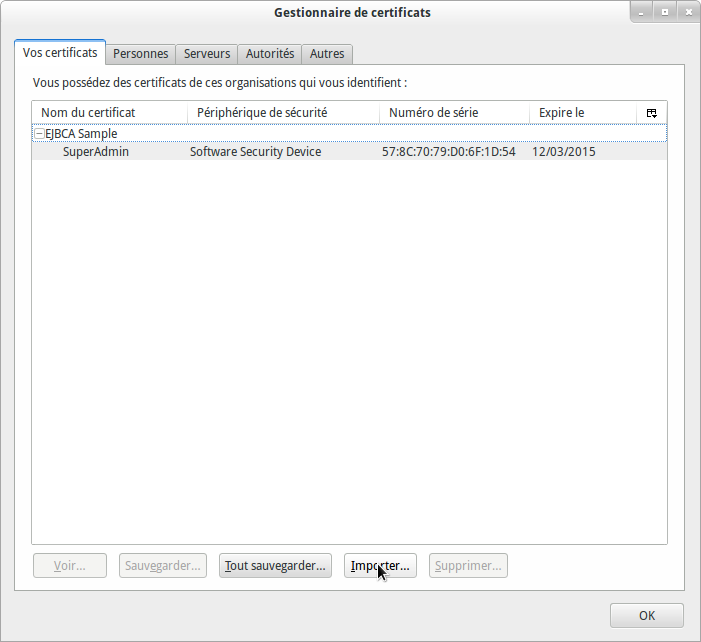
\includegraphics[width=30em]{import_superadmin.png}
\end{center}

On peut alors accéder à la partie administration à partir de l'adresse:

\verb+https://adresse_serveur:8443/ejbca/adminweb/index.jsp+
\newpage
La page obtenue est la suivante :
\begin{center}
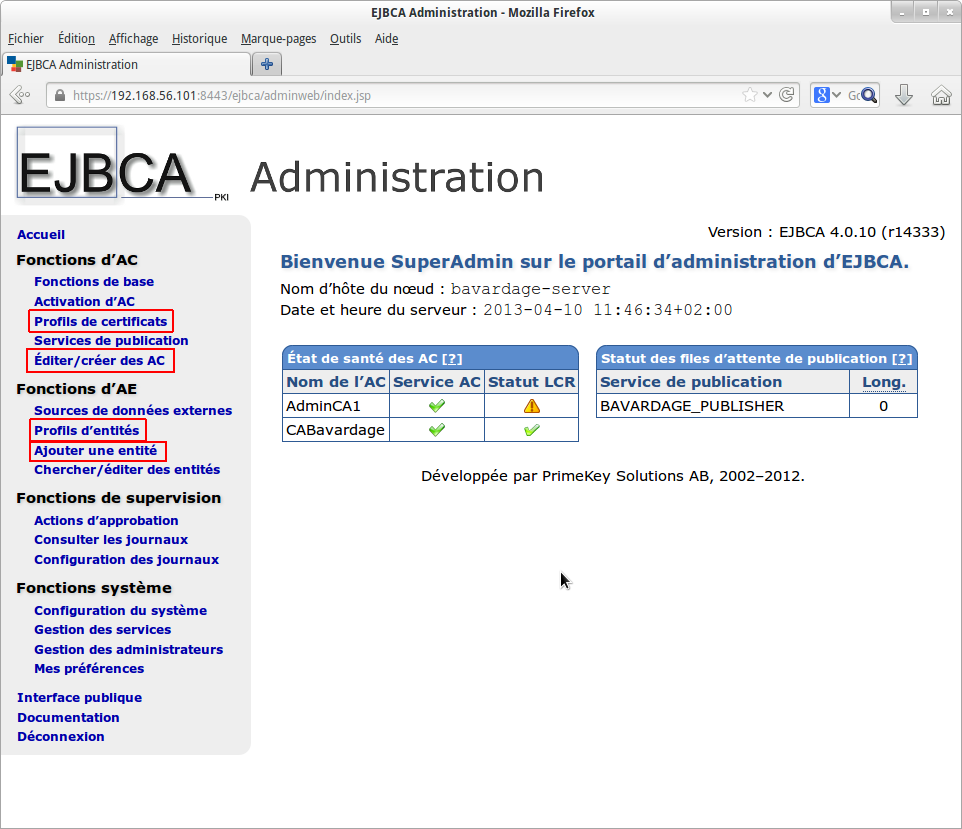
\includegraphics[width=40em]{admin_ejbca.png}
\end{center}

Les parties importantes ont été entourées en rouge et voici leurs descriptions.

\begin{paragraph}{Profils de certificats}
C'est dans cette section que l'ont créer les différents profils de certificats :
\begin{itemize}
\item \verb+BAVARDAGESERVER+ : profil pour le serveur sécurisé ;
\item \verb+BAVARDAGEUSER+ : profil pour les utilisateurs sécurisés.
\end{itemize}

Ces profils sont décrits en détail dans le document annexe : Politique de certification
\end{paragraph}

\begin{paragraph}{Éditer/créer des AC}
Une AC (autorité de certification) est une entité dont la mission est de vérifier les données du demandeur de certificat, de signer et de maintenir une liste des certificats et une liste des révocations. Sur la capture d'écran ci-dessus, on voit la liste des AC contenant celle relative à notre projet : \verb+CABavardage+
\end{paragraph}


\begin{paragraph}{Profils d'entités}
Chaque type d'entité a un profil associé:
\begin{itemize}
\item \verb+BAVARDAGE_SERVER+ : profil pour le serveur sécurisé ;
\item \verb+BAVARDAGE_USER+ : profil pour les utilisateurs sécurisés.
\end{itemize}
\end{paragraph}


\begin{paragraph}{Ajouter une entité}
Lorsqu'un utilisateur désire obtenir un certificat, un administrateur doit au préalable lui crée une entité associée. Il pourra ensuite récupérer son certificat pour sa clef RSA.
\end{paragraph}


\subsection{Partie sécurisée}
La troisième livraison consistait en la surcouche sécurisée du client de chat et d'un serveur « sécurisé » dont le rôle est de gérer les utilisateurs sécurisés.

Il a tout d'abord fallu ouvrir une connexion SSL entre le client sécurisé et le serveur sécurisé grâce aux fonctions d'OpenSSL. Ensuite, nous avons créer des codes d'actions spécifiques à l'utilisation sécurisée du chat comme \verb+CONNECT_SEC, CREATE_ROOM_SEC+... La gestion des clients dans le serveur sécurisé est similaire au serveur classique avec un fil d'exécution par client et une socket SSL.

Côté client, la surcouche sécurisée se base sur la librairie du client classique et utilise la même logique. Ainsi nous avons deux fonctions principales : 
\begin{itemize}
\item \verb+int send_message_sec (const char *mess, char **err_mess)+
\item \verb+int receive_message_sec (message *m)+
\end{itemize}

On rajoute également des fonctions de chiffrement/déchiffrement de messages :
\small{
\begin{itemize}
\item \verb+char *aes_encrypt (unsigned char *key, unsigned char *iv, char *plaintext, int *len)+

\item \verb+char *aes_decrypt (unsigned char *key, unsigned char *iv, char *ciphertext, int *len)+
\end{itemize}
}

Pour le chiffrement et le déchiffrement nous utilisons une fonction \\
 \verb+char *gen_keyiv(key_iv keyiv, unsigned char *key_data, int key_data_len)+ 
 qui génère la clé et l'IV. C'est cette paire (clé,iv) qui est utilisée par les fonctions \verb+aes_encrypt+ et \verb+aes_decrypt+ pour chiffrer et déchiffrer les messages.

Comme les noms des fonctions l'indiquent, nous utilisons AES-256-CBC pour chiffrer les messages envoyés (champ \verb+content+). AES est un chiffrement par bloc qui supporte des clés et des blocs de 128, 192 et 256 bits. Le mode de chiffrement CBC consiste à diviser les données en plusieurs blocs de même taille et à les chiffrer de manière chaînée (le résultat précédent est utilisé lors du chiffrement suivant). L'IV est utilisé pour le chiffrement du premier bloc. Avec le mode CBC l'IV est unique et aléatoire,ce qui rend la clé réutilisable sans risque, et il n'y a pas de risque de répétition de bloc. Nous avons choisi AES-256-CBC pour avoir une plus grande taille des clés et la sécurité qu'offre le mode de chiffrement CBC. 


\section{Problèmes rencontrés}
Nous avons rencontré un problème pour la livraison du sprint 2. En effet, nous devions configurer un serveur, ce que nous avions fait dans une machine virtuelle. Cependant, le format de livraison utilisé jusqu'alors n'était plus utilisable car la machine faisait plusieurs giga octets de données. Nous avons alors convenu avec Mme Bardet de livrer sur une clef USB dans un premier temps et de configurer une machine mise à disposition par Mr Macadré.

Pour le sprint 3, nous avons eu également eu des problèmes au niveau de l'apprentissage d'OpenSSL. En effet, nous n'avions aucune expérience avec cette bibliothèque et les exemples sont nombreux mais très différents. Finalement, Mme Bardet nous a conseillé un très bon ouvrage : Network Security with OpenSSL.
OpenSSL



\newpage
%%%%%%%%%%%%%%%%%%%%%%%%%%%%%%%%%%%%%%%%%%%%
% MANUEL D'UTILISATION 
% Charles & Ismaël
%%%%%%%%%%%%%%%%%%%%%%%%%%%%%%%%%%%%%%%%%%%%
\chapter{Manuel d'utilisation}
\section{Récupération du projet}
 Les sources du projet sont disponibles sur un dépôt git. Elles peuvent être récupérées en ligne de commande ou en ligne. 
 
 \subsection{En ligne de commande}
 Placez vous dans un terminal et exécutez la commande suivante :
\begin{verbatim} 
    $ git clone git://github.com/legrajul/bavardage.git 
\end{verbatim}

\subsection{En ligne}
 Une archive contenant le projet peut être téléchargé à l'adresse :

\section{Compilation}
\subsection{Dépendances Ubuntu}
Pour la compilation du projet il faut d'abord vérifier si toutes les dépendances sont satisfaites :
\begin{itemize}
\item cmake : permet de compiler un projet pour différentes plateformes.
\item valac-0.18 : compilateur Vala qui traduit le code source vala en code source C.
\item libgtk-3-dev : outil multi plateformes pour créer des interfaces graphiques.
\item libgee-dev : librairies de collections fournissant des classes basées sur GObject.
\item libglib2.0-dev : fichiers de développement pour la bibliothèque GLib.
\item libssl-dev : bibliothèque de développement SSL.
\item libsqlite3-dev : bibliothèque de développement SQLite.

\end{itemize}

\subsection{Compilation des sources}

Les commandes suivantes doivent être exécuter dans le dossier du projet git bavardage : 
\begin{verbatim}
    $ mkdir src/build 
    $ cd src/build 
    $ cmake .. 
    $ make
\end{verbatim}

\section{Exécution}

\subsection{Serveur non sécurisé}
Pour lancer le serveur non sécurisé, il faut d'abord se rendre dans le répertoire "server" du répertoire build et taper les instructions suivantes:

\begin{verbatim}
    $ ./server ADRESSE_SERVEUR PORT_SERVEUR
\end{verbatim}

\verb+ADRESSE_SERVEUR+: l'adresse IP ou le nom de domaine du serveur non sécurisé

\verb+PORT_SERVEUR:+ le numéro du port d'écoute du serveur

\subsection{Serveur sécurisé}
Pour lancer le serveur sécurisé, il faut d'abord se rendre dans le répertoire "serversec" du répertoire "build" et taper les instructions suivantes:
\begin{verbatim}
    $ ./serversec ADRESSE_SERVEUR_SEC PORT_SERVEUR_SEC
\end{verbatim}

\verb+ADRESSE_SERVEUR_SEC+: l'adresse IP ou le nom de domaine du serveur sécurisé

\verb+PORT_SERVEUR_SEC+: le numéro du port d'écoute du serveur sécurisé

\subsection{Client}
Pour lancer le client, il faut se rendre dans le répertoire "client" du répertoire "build" et lancer les instrutions suivantes:
\begin{itemize}
\item Client console : 
\begin{verbatim}
    $ ./clientsec-cli ADRESSE_SERVEUR PORT_SERVEUR ADRESSE_SERVEUR_SEC PORT_SERVEUR_SEC CERTIFICAT CLE_PRIVEE [MOT_DE_PASSE_CLE]
    $ ./clientsec-cli CERTIFICAT CLE_PRIVEE [MOT_DE_PASSE_CLE]
\end{verbatim}
\item Client Graphique :
\begin{verbatim}
    $ ./Client
\end{verbatim}
\end{itemize}

\verb+ADRESSE_SERVEUR+: l'adresse IP ou le nom de domaine du serveur non sécurisé.

\verb+PORT_SERVEUR+: le numéro du port d'écoute du serveur.

\verb+ADRESSE_SERVEUR_SEC+: l'adresse IP ou le nom de domaine du serveur sécurisé.

\verb+PORT_SERVEUR_SEC+: le numéro du port d'écoute du serveur sécurisé.

\verb+CERTIFICAT+: le chemin d'accès au certificat délivré par l'autorité de certification.

\verb+CLE_PRIVE+: la clé privée générée par l'utilisateur

\verb+MOT_DE_PASSE_CLE+: le mot de passe de la clé privée si elle a été généré avec un mot de passe.

	Concernant le client console, la deuxième commande est utilisée lorsque l'adresse et le port du serveur sécurisé/non sécurisé sont celles par défaut (adresse/port serveur: localhost/10000, adresse/port serveur sécurisé: localhost/11000).
	
\subsection{Utilisation du client console}
	
	La forme générale des commandes est : 
	
\verb+ /NOM_COMMANDE [paramètre_1 [Paramètre_2 [Paramètre_3 Paramètre_4]]]+

La commande de base de l'application est /HELP. Elle permet de lister toutes les autres commandes de l'application.
\subsubsection{Commandes du client classique et les actions}

\verb+	/CREATE_ROOM room_name+  : Permet de créer un salon ayant le nom "room\_name"

\verb+	/DELETE_ROOM room_name+ :  Permet de supprimer le salon du nom de "room\_name"

\verb+	/QUIT_ROOM room_name+ :  Permet de quitter le salon du nom de "room\_name"

\verb+	/JOIN_ROOM room_name+:  Rejoindre un salon du nom de "room\_name"

\verb+	/DISCONNECT+: Se déconnecter du serveur non sécurisé

\verb+	/CONNECT user+:  Se connecter avec l'identifiant "user"

\verb+	/MP user message+: Envoyer un message privé à l'utilisateur "user"
			
\subsubsection{Commandes du client sécurisé et les actions}

\verb+	/CONNECT_SEC user user_certif user_key+: Connexion au serveur sécurisé avec le nom d'utilisateur "user" avec le certificat "user\_certif" et la clé privée "user\_key" (Si la clé privée a été crée avec un mot de passe, il faut ajouter le mot de passe après "user\_key")

\verb+	/CREATE_ROOM_SEC room_name+: Permet de créer un salon sécurisé du nom de "room\_name"

\verb+	/DELETE_ROOM_SEC room_name+: Permet de supprimer le salon sécurisé du nom "room\_name"

\verb+	/DISCONNECT_SEC+: Se déconnecter du serveur sécurisé et du serveur non sécurisé

\verb+	/QUIT_ROOM_SEC room_name+: Quitter le salon sécurisé du nom de "room\_name"

\verb+	/JOIN_ROOM_SEC room_name+: Rejoindre le salon sécurisé du nom de "room\_name"

\verb+	/DEL_ACCOUNT_SEC+: Supprimer le compte utilisateur sécurisé

\verb+	/MP_SEC user message+: Envoyer un message privé sécurisé

\verb+	/MESSAGE room_name message+: Envoyer le message "message" à "user" ou sur le salon "room\_name"

\verb+	/ACCEPT_JOIN_ROOM_SEC room_name user+: Accepter la requête d'ajout qu'un utilisateur a envoyé pour rejoindre un salon. Seul l'administrateur du salon a les droits pour effectuer cette opération.

\verb+	/REFUSE_JOIN_ROOM_SEC room_name user+: Refuser la requête d'ajout qu'un utilisateur a envoyé pour rejoindre un salon. Seul l'administrateur du salon a les droits pour effectuer cette opération.

\verb+	/EJECT_FROM_ROOM_SEC room_name user+: Supprimer un utilisateur "user" du salon "room\_name". Seul l'administrateur du salon a les droits pour effectuer cette opération.


\subsection{Utilisation du client graphique}

Le client graphique permet d'effectuer les mêmes opérations que le client console mais avec l'intuitivité que nous offre l'interface graphique.

\subsubsection{Connexion non sécurisée}
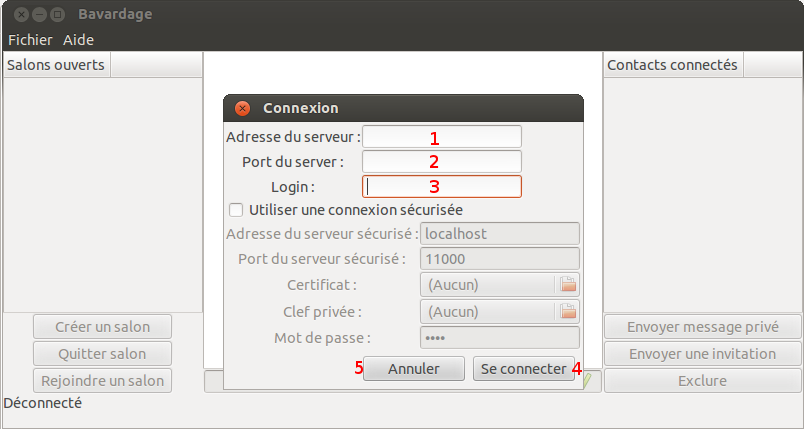
\includegraphics[width=45em]{capture/con_n_sec.png}

Pour effectuer une connexion non sécurisée, il faut:
\begin{enumerate}
    \item Entrer l'adresse du serveur non sécurisé;
    \item Entrer le port d'écoute du serveur non sécurisé;
    \item Entrer le login voulu pour se connecter;
    \item Cliquer sur le bouton "Se connecter" pour lancer la connexion;
    \item Cliquer sur le bouton "Annuler" pour annuler la connexion;
\end{enumerate}
\subsubsection{Connexion sécurisée}

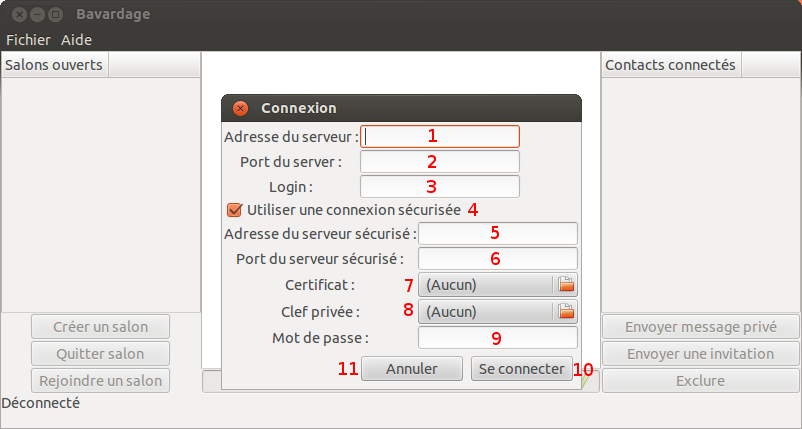
\includegraphics[width=45em]{capture/con_sec.png}

Pour effectuer une connexion sécurisée, il faut:

\begin{enumerate}
    \item Entrer l'adresse du serveur non sécurisé;
    \item Entrer le port d'écoute du serveur non sécurisé;
    \item Entrer le login voulu pour se connecter;
    \item Cocher l'option de connexion sécurisée;
    \item Entrer l'adresse du serveur sécurisé;
    \item Entrer le port d'écoute du serveur sécurisé;
    \item Sélectionner le fichier du certificat délivré par l'autorité de certification;
    \item Sélectionner le fichier de la clé privée;
    \item Entrer le mot de passe correspondant à la clé privée (Si aucun mot de passe n'a été utilisé pour générer la clé privée, ne rien entrer dans ce champ);
    \item Cliquer sur le bouton "Se connecter" pour lancer la connexion;
    \item Cliquer sur le bouton "Annuler" pour annuler la connexion;
\end{enumerate}

\subsubsection{Création d'un salon (sécurisé ou non sécurisé)}

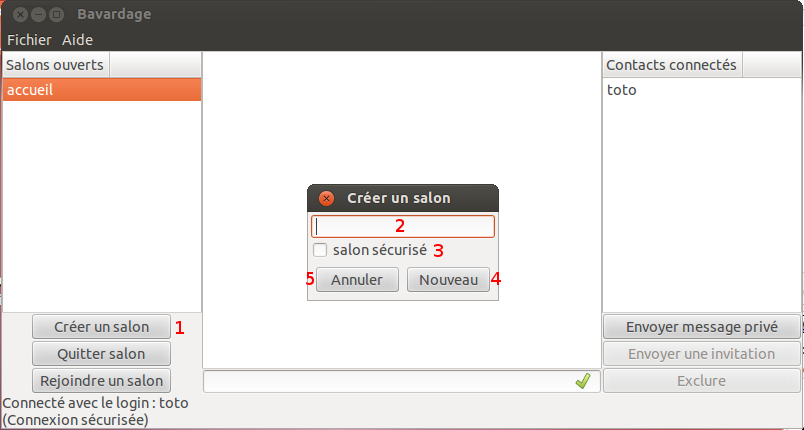
\includegraphics[width=45em]{capture/cre_room.png}

Pour effectuer la création d'un salon (sécurisé ou non sécurisé), il faut:
\begin{enumerate}
    \item Cliquer sur le bouton "Créer un salon";
    \item Entrer le nom du salon à créer dans le champ;
    \item Cocher le champ "salon sécurisé" s'il s'agit d'un salon sécurisé;
    \item Cliquer sur le bouton "Nouveau" pour créer le salon;
    \item Cliquer sur le bouton "Annuler" pour annuler la création du salon.
\end{enumerate}

\subsubsection{Rejoindre un salon (sécurisé ou non sécurisé)}

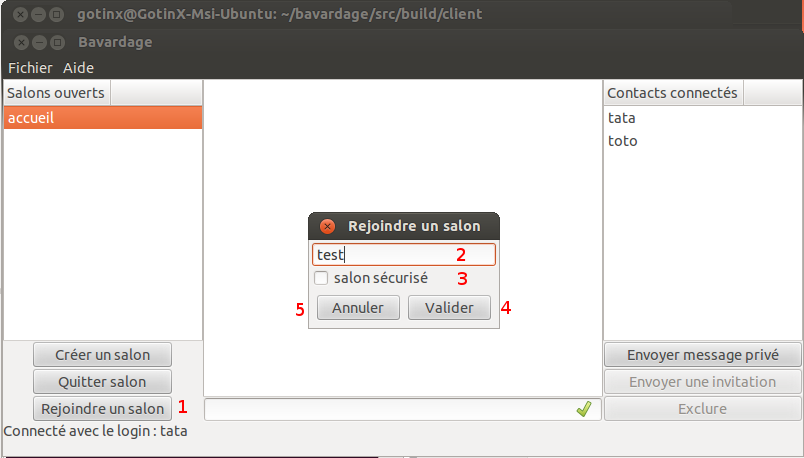
\includegraphics[width=45em]{capture/rej_sal.png}

Pour rejoindre un salon (sécurisé ou non sécurisé), il faut:

\begin{enumerate}
    \item Cliquer sur le bouton rejoindre un salon;
    \item Entrer le nom du salon à rejoindre;
    \item Cocher la case "salon sécurisé";
    \item Cliquer sur le bouton "Se connecter" pour rejoindre le salon s'il n'est pas sécurisé ou envoyer une demande à l'administrateur du salon si le salon est sécurisé;
    \item Cliquer sur le bouton "Annuler" pour annuler la connexion.
\end{enumerate}

\subsubsection{Envoyer un message dans un salon}

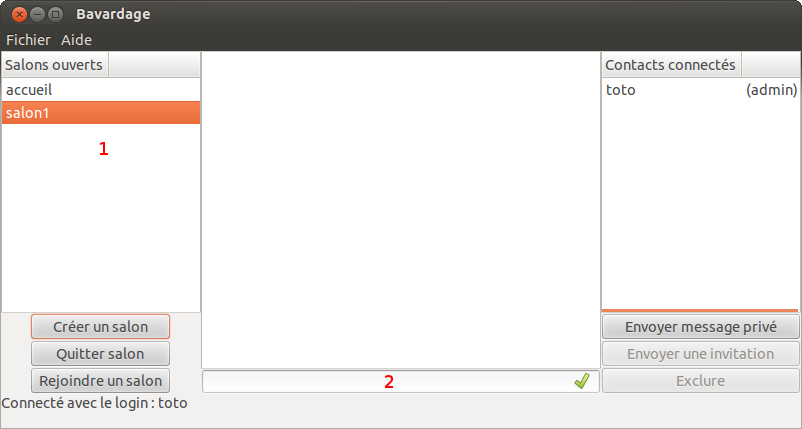
\includegraphics[width=45em]{capture/mess_room.png}

Pour envoyer un message dans un salon, il faut:
\begin{enumerate}
    \item Sélectionner le salon dans lequel on veut envoyer le message dans la liste des salons ouverts;
    \item Saisir le message dans la zone puis appuyer sur la touche "Entrée" pour envoyer le message.
\end{enumerate}

\subsubsection{Envoyer un message privé à un utilisateur}

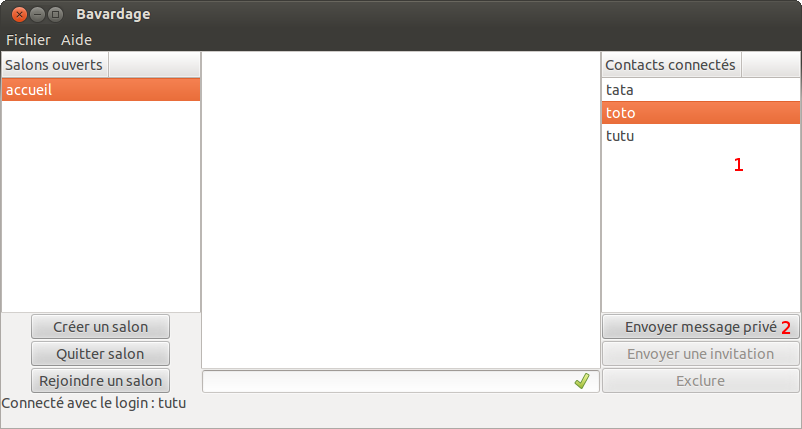
\includegraphics[width=45em]{capture/mp_nsec.png}

Pour envoyer des messages en mode privé à un utilisateur, il faut:

\begin{enumerate}
    \item Sélectionner l'utilisateur dans la liste des contacts connectés;
    \item Cliquer sur le bouton "Envoyer message privé".
    \item Une boite de dialogue s'afficher pour demander si l'on veut une discussion sécurisée avec l'utilisateur 
\end{enumerate}

\subsubsection{Accepter la requête d'un utilisateur qui souhaite rejoindre un salon}

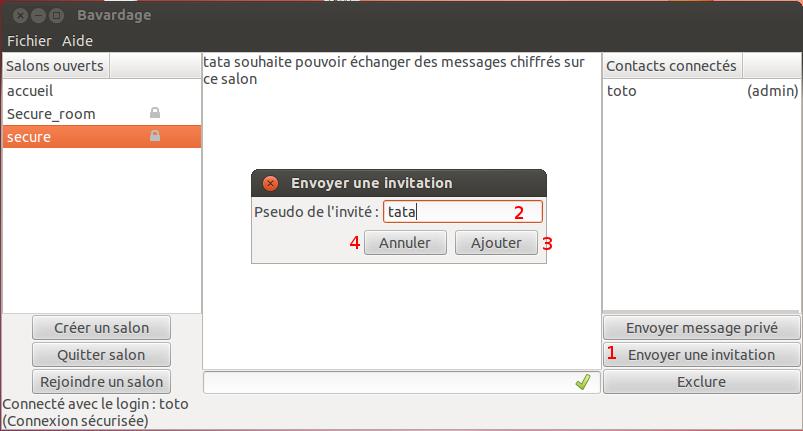
\includegraphics[width=45em]{capture/invit_room.png}

Pour accepter une demande d'invitation reçu,
\begin{enumerate}
    \item Cliquer le bouton "Envoyer une invitation";
    \item Entrer le pseudo de l'utilisateur ayant envoyé la demande;
    \item Cliquer le bouton "Ajouter" pour rajouter l'utilisateur au salon sécurisé
    \item Cliquer sur le bouton "Annuler" pour annuler l'ajout de l'utilisateur
\end{enumerate}

\subsubsection{Exclure un utilisateur}
Pour exclure un utilisateur,
\begin{enumerate}
    \item Sélectionner le pseudo de l'utilisateur dans la liste des contacts connectés;
    \item Cliquer sur "Exclure".
\end{enumerate}

\subsubsection{Quitter un salon}

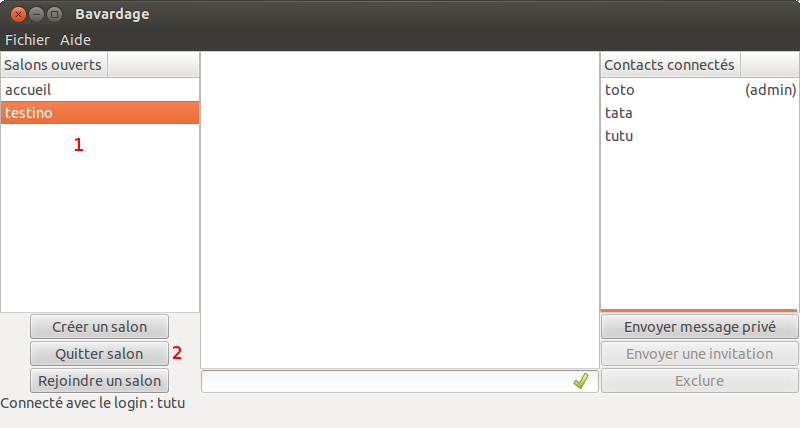
\includegraphics[width=45em]{capture/quit_room.png}

Pour quitter un salon, il faut:

\begin{enumerate}
    \item Sélectionner le salon que l'on veut quitter dans la liste des salons ouverts;
    \item Cliquer sur le bouton "Quitter salon".

\end{enumerate}

\subsubsection{Se déconnecter}
Pour se déconnecter,
\begin{enumerate}
    \item Aller dans le menu "Fichier";
    \item Cliquer sur "Déconnecter".
\end{enumerate}

\newpage
%%%%%%%%%%%%%%%%%%%%%%%%%%%%%%%%%%%%%%%%%%%%
% CONCLUSION 
% JB
%%%%%%%%%%%%%%%%%%%%%%%%%%%%%%%%%%%%%%%%%%%%
\frontmatter
\pagestyle{fancy}
\large
\chapter{Conclusion}

Ce projet a été découpé en deux parties distinctes, l'analyse et l'étude d'un sujet associé à une gestion de projet
afin de proposer une solution au client puis une deuxième phase qui a été 
l'implémentation de la solution proposée également accompagné d'une gestion de 
projet.

L'étude et l'analyse théorique du sujet lors de la première phase de projet nous a permis
d'apprendre à mettre en place des documents spécifique et détaillés sur chaque fonctionnalités en utilisant des méthodes de conception 
professionnelle. La méthode agile, scrum, que nous avons choisi a permis d'établir un planning de gestion et un découpage astucieux du projet en plusieurs
étapes et ainsi proposer une solution structurée respectant au mieux les besoins du client.

La deuxième phase, d'implémentation, a été un moyen de mettre en pratique 
nos techniques de programmation acquise au cours de nos formations antérieur, nos connaissances théorique en cryptographie
mais également d'apprendre de nouvelles technologie en particulier pour la mise en place des techniques de cryptographie 
et la gestion d'une autorité de certification avec certificats dans une application concrète et fonctionnelle.

La méthode agile, scrum, utilisé pour ce projet, a simplifié les phases afin d’en raccourcir la durée.
Les méthodes agiles, se basent sur la notion de communauté de projet dans laquelle les développeurs
et les utilisateurs sont présents en permanence pour exprimer ou répondre à une question liée au projet. 
C'est une communication permanente entre les membres du groupe de projet, et le client qui a fait que 
nous avons su rapidement, prendre en compte les opinions et idées de chacun et de réagir aux 
différents problèmes que ce soit lors de l'analyse ou de l'implémentation du 
projet. Nous en tirons donc une expérience très enrichissante sur la gestion et 
la communication au sein d'un groupe de projet dans un cadre orienté professionnel.



\newpage
\appendix
\chapter{Documents de gestion de projet}
\chapter{Déclaration des pratiques de certification}
\section{Introduction}
\subsection{Contexte Général}
La PKI mise en place pour le projet de chat sécurisé fournit des certificats (Durée : 2 ans) aux utilisateurs sécurisés du chat.
Ces certificats sont utilisés sur le chat pour s'authentifier.

\subsection{Délégation d'autorité d'enregistrement}
Pas de délégation du rôle d’Autorité d’Enregistrement dans notre cas. La PKI assurera ce rôle.

\subsection{Souscripteur}
Le souscripteur est l’utilisateur du chat souhaitant se connecter au chat sécurisé. Le souscripteur est identifié dans chaque certificat. Une fois acceptée, l’adhésion au service pour le souscripteur est valable pour la totalité de la période de validité du certificat sauf révocation.

\section{Pré requis pour les demandes}
\subsection{Enregistrement d'un souscripteur}
\begin{itemize}
\item Le souscripteur fournit à la RA toutes les informations nécessaires à son enregistrement. 
\item Le souscripteur s'engage à fournir des informations correctes et précises et avertir la RA en cas de mise à jour nécessaire de ces informations tout au long de la période de validité du certificat par le moyen de communication le plus adapté.
\end{itemize}

\subsection{Vérification}
L’AE doit :
\begin{itemize}
\item Vérifier le remplissage correct de tous les champs par le souscripteur en respectant les conventions.
\item Enregistrer le souscripteur.
\item Transmettre la demande à la CA.
\end{itemize}
L’AE a le droit de refuser toute demande.

\section{Pratiques et procédures}
\subsection{Demande de certificats}
Lorsque l'utilisateur fait une demande de certificat, la RA vérifie si les informations respectent les conventions, si les données
respectent, la demande est automatiquement envoyée à l'autorité de certification pour génération du certificat. La demande se fait via un formulaire disponible sur l'application cliente du chat.

\subsection{Validation  des demandes}
Le délai moyen entre la réception des demandes complètes et la délivrance d'un certificat est de 1 jour. En cas de non validation des informations, la RA rejette la demande. Le demandeur peut refaire sa demande suite à un rejet.

\subsection{Révocation des certificats}
La révocation entraîne la fin de validité du certificat avant la date de fin initialement prévue. La RA vérifie que la demande de révocation est :
\begin{itemize}
\item Soit faite par l'utilisateur ayant fait la demande de certificat :  la demande de révocation sera traitée.
\item Soit faite par une entité disposant des droits nécessaires: la RA révoquera le certificat. La demande de révocation et l'identité de l'entité seront conservées.
\end{itemize}

\subsection{Expiration}
La PKI doit s'efforcer de prévenir le souscripteur par email, 30 jours avant l'expiration de son certificat.

\subsection{Renouvellement}
Idem que pour demande de certificat.

\section{Conservation et Protection des données}
La PKI conserve les données relatives aux certificats pendant 2 ans minimum après expiration ou révocation des certificats. La PKI garde des copies des certificats quel que soit leur statut et conserve les logs pendant une période de 2 ans ou pour une période conforme à la loi. 
\\La PKI respecte les règles applicables sur la protection des données personnelles jugées par la loi comme confidentielles.


\newpage
\textbf {Acronymes}


\begin{tabular}{|l|p{10cm}|}

\hline
CA & Certification Authority
\\
\hline
AE  & Registration Authority 
\\

\hline
DPC & Déclaration des Pratiques de Certification
\\
\hline
PKI & Public Key Infrastructure
\\
\hline
CNRS & Centre National de la Recherche Scientifique
\\
\hline
TCS & Terena Certificate Service
\\
\hline
\end{tabular}



\newpage
\textbf {Documents applicables et de référence}
\begin{itemize}
\item PC (Politique de certification)
\item Déclaration des pratiques de certification TCS (CNRS)

\end{itemize}




\chapter{Politique de certification}
\section{Introduction}
\subsection{Présentation générale}

Le groupe F du Master professionnel 1 SSI (2012-2013), dans le cadre de son projet annuel doit étudier et réaliser un outil de chat sécurisé. L'objectif de ce projet est d'étudier les protocoles cryptographiques permettant à plusieurs utilisateurs de s'authentifier et de communiquer de manière sécurisée à travers un outil de messagerie instantanée.


\subsection{ Identification }

Ce document est la politique de certification du chat sécurisé Bavardage et est identifié par le nom Bavardage-pc.


\subsection{ Autorités, applications et groupes d'utilisateurs concernés }
\subsubsection{Autorité administrative (AA)}

Composante de la PKI qui définit et fait appliquer les politiques de certification et les déclarations des pratiques de certification par la PKI.
	
\subsubsection{Autorité de certification (CA)}
C'est l'autorité à laquelle les utilisateurs font confiance pour gérer les certificats(générer, publier, révoquer), et les révocations. Le CA est gérée par l'administrateur du serveur sécurisé du chat. Le Common Name du CA sera BavardageCA.


\subsubsection{Autorité d'enregistrement (RA)}

Une autorité d’enregistrement est une composante de la PKI qui vérifie les données propres au demandeur de certificat ainsi que les contraintes liées à l’usage d’un certificat, conformément à la politique de certification. Elle assure le lien entre l'Autorité de Certification et les utilisateurs. 

\subsubsection{Autorité de dépôt (AD)}
C'est l'autorité qui stocke les certificats numériques ainsi que les listes de révocation.

\subsubsection{ Utilisateur demandeur (UD)}

C'est la personne physique ayant directement par la loi ou par délégation, le pouvoir de demande de certificat portant le nom du chat et du signataire de la convention.

\subsubsection{ Utilisateur Final (UF)}

C'est la personne physique qui utilise les certificats. C'est un utilisateur du chat.

\subsubsection{Utilisateur signataire convention (USC)}

C'est la personne physique ayant directement par la loi ou par délégation, le pouvoir de signer les conventions passées avec Bavardage. Tous les certificats porteront le nom du chat et le nom du signataire de la convention passée bavardage. 
		
\subsubsection{Type d'applications concerné}

L'usage des certificats doit permettre l'authentification d'un utilisateur. Bavardage décline toute responsabilité pour tout usage de certificat qui serait sans rapport avec le chat.

\subsection{Points de contact}
\subsubsection{Autorité de sécurité compétente dans l'accréditation des composants d'une PKI}
		À compléter
		
\subsubsection{Personnes à contacter concernant ce document}		
Toute personne desirant contacter Bavardage concernant ce document peut envoyer un mail à l'adresse bavardage@gmail.com.

\subsubsection{Personnes habilitées à déterminer la conformité de la DPC avec la PC}

Les personnes habilitées à déterminer la conformité de la DPC avec la PC sont nommées par l’Autorité Administrative(AA).

\section{Dispositions d'ordre générale}
\subsection{Obligations}
Les obligations suivantes sont communes à toutes les composantes de la PKI:
Protéger sa clé privée et ses données d’activation en intégrité et en confidentialité.
N’utiliser ses clés publiques et privées qu’aux fins pour lesquelles elles ont été émises et avec les outils spécifiés, en vertu de la présente politique.
Respecter et appliquer la PC.
Mettre en œuvre les moyens (techniques et humains) nécessaires à la réalisation des prestations auxquelles l’entité concernée s’engage.

\subsubsection{Obligations des acteurs}
\begin{tabular}{|l|p{10cm}|}
  \hline
  Autorité Administrative &  
  \begin{itemize}
   \item Valider la politique de certification
   \item Établir la conformité entre la PC et la DPC
   \end{itemize}

 \\
  \hline
  Autorité d'Enregistrement & 
  \begin{itemize}
  \item  Respecter la législation relative au respect des données
d’identification personnelles
\item Publier un formulaire de demande de certification.
\item Vérifier l'exactitude des mentions qui établissent l'identité du
demandeur.
\item Si elle est saisie d'une demande de révocation, elle doit en vérifier l'origine et l'exactitude.
\item Traiter les demandes de certificat.
\item Conserve et protège en confidentialité et intégrité toutes les données collectées lors de la demande de certificat.
\item Doit se soumettre à tout contrôle technique et audits que pourrait demander l'AA.
  \end{itemize}
  \\
  \hline
  Autorité de Certification &
  \begin{itemize}

\item S'engager à diffuser publiquement la politique de certification, la liste des certificats révoqués, et la liste des certificats.
\item Respecter le résultat d’un contrôle de conformité et remédier aux non conformités qu’il révèle
\item Documenter ses procédures internes de fonctionnement.
\item Respecter la PC et appliquer la DPC.
\item Doit se soumettre à tout contrôle technique et audits que pourrait demander l'AA.

  \end{itemize}
 \\
 \hline
 Utilisateur Demandeur &
 \begin{itemize}
 \item Il doit respecter la convention avec le chat bavardage et la PC

 
 \end{itemize} 
  
 \\
 \hline
 Utilisateur Final &
 \begin{itemize}
 \item Se conformer aux règles de la présente politique de certification.
\item Respecter les conditions d'utilisation des clés et certificats, et protéger ceux-ci.
\item A défaut de remplir cette obligation il assume seul tous les risques de ses actions non conformes aux exigences de la présente politique.
 
 \end{itemize}
\\
\hline
  
\end{tabular}
\subsubsection{Responsabilité des acteurs}

\begin{tabular}{|l|p{10cm}|}
  \hline
  Autorité Administrative &  
  \begin{itemize}
  \item Résolution des litiges
   \end{itemize}

 \\
  \hline
  Autorité d'Enregistrement & 
  \begin{itemize}
\item Enregistrement d’une demande en provenance des utilisateurs (UD).
\item Conservation et protection en confidentialité et en intégrité des données personnelles d’identification transmises pour l’enregistrement.
\item Seule la CA peut mettre en cause la responsabilité de la RA, ce qui exclut explicitement tout engagement de la RA envers les utilisateurs demandeurs ou finaux.

  \end{itemize}
  \\
  \hline
  Autorité de Certification &
  \begin{itemize}
\item Génération des certificats dans le cadre des procédures définies dans la PC et DPC.
\item Assure la responsabilité du service de publication, elle est responsable de l'information des utilisateurs des procédures à suivre tout au long du cycle de vie des certificats.


  \end{itemize}
 \\
 \hline
 Utilisateur Demandeur &
 \begin{itemize}
\item Il réalise les opérations de demande et révocation de certificats.
 
 \end{itemize} 
  
 \\
 \hline
 Utilisateur Final &
 \begin{itemize}
\item Il est responsable de la sécurité de son poste de travail (clefs et certificats).
 
 \end{itemize}
\\
\hline
  
\end{tabular}             

\subsubsection{Interpretation de la loi}
\begin{itemize}
\item Loi
Suivant la législation nationale :
Les données à caractère personnel d’une personne physique doivent être protégées suivant la loi.

\end{itemize}

\subsubsection{Publication et Services associés}
\begin{itemize}

\item Publication d’informations sur la PKI

Les informations concernant la PKI publiées sont les suivantes :
\begin{itemize}
\item La Politique de certification (PC)
\item La liste des certificats révoqués(LCR)
\end{itemize}

\item Fréquence de publication
\\Les informations seront publiées suivant un temps T

\item Service de publication
\\La CA rend un service de publication des certificats qui se matérialisera par un annuaire. Ce service de publication met à disposition des utilisateurs suivant TEMPS=TempDispoPub les informations suivantes :
\begin{itemize}
\item les informations concernant la PKI
\item la liste des certificats révoqués
\end{itemize}

\end{itemize}

\subsubsection{Contrôle de conformité}
À compléter

\subsubsection{Politique de confidentialité}
\begin{itemize}
\item Type d'informations considérées comme confidentielles

Cas des informations confidentielles à caractère secret (obligation de discrétion). Il s’agit d’informations nécessaires au bon fonctionnement de la PKI :
\begin{itemize}

\item La DPC
\\
\end{itemize}



Cas des informations confidentielles à caractère privatif (exigence de séclusion). Il s’agit d’informations nécessaires à l’opérabilité de la PKI :
données personnelles d’identification nominative d’un utilisateur demandeur (identifiants nominatifs), les utilisateurs demandeurs disposent d'un droit d'accès, de rectification et d'opposition à la cession de toute information les concernant.
\\

\item Type d'informations considérés comme non confidentielles
\\Les informations publiées sur la PKI (cf. 2.1.4) sont considérées comme non confidentielles.
\\
\item Delivrance aux autorités légales
\\les autorités légales peuvent réclamer l’identité de l’individu ou de l’organisme qu’il représente. En aucun cas, le recouvrement de clé de signature ni de clé de certification ne doit être effectué.
\\

\item Delivrance à la demande du propriétaire
\\Les informations relatives à un utilisateur final et définies comme confidentielles (cf. 2.1.2) ne peuvent être divulguées qu’à leur propriétaire (demandeur du certificat).
\end{itemize}

\section{Identification et authentification}
\subsection{Enregistrement initial}
\subsubsection{Convention}
La convention est le règlement que tout detenteur du certificat doit respecter. Seul l'UD peut signer la convention. Il doit obligatoirement se présenter physiquement à l'AA pour signer la convention.

\subsubsection{Convention de noms}
Le nom de l'Abonné figure dans le champ "Nom de l'organisation" du certificat au format X.509. Cette mention est obligatoire. Il est constitué du prénom usuel et du nom usuel. Ce nom est celui de l'Abonné tel qu'il figure dans les documents d'État Civil.

\subsubsection{Nécessité d'utilisation de noms explicites}

Les informations portées dans les champs du certificat CA Certificat sont décrites ci-dessous de manière explicite :
\begin{itemize}
\item Pays : le code du pays sur 2 lettres
\item Mot de passe : requis pour la signature
\item Password : confirmation du mot de passe
\item Etat ou nom de province : 
\item Localité : la ville
\item Nom de l'organisation: Nom de l'entreprise ou de la personne
\item Unité organisationnelle : departement
\item Adresse eMail : Adresse électronique de l'abonné

\end{itemize}

\subsubsection{Règles d'interprétation des différentes formes de nom}
Ces informations sont établies par le groupe de projet et reposent essentiellement sur les règles
suivantes :
\begin{itemize}
\item Tous les caractères sont sans accents ni caractères spécifiques à la langue française;
\item les prénoms et noms composés sont séparés par des tirets " - ".

\end{itemize}

\subsubsection{Unicité des noms}
L’unicité d’un certificat est basée sur l’unicité de son numéro de série au sein de la CA et du nom de l'abonné.

\subsubsection{Procédures de résolution des litiges sur la révendication d'un nom}
Lorsque le nom à inclure dans un certificat provoque un litige avec un autre utilisateur, l’autorité d’enregistrement à qui la demande de certification a été formulée proposera une procédure de résolution amiable du litige.

\subsubsection{Preuve de la possession d'une clé privée}
Génération du bi-clé par le demandeur et utilisation d'un protocole adapté.

\subsubsection{Authentification de l'identité d'un individu}
L'authentification d'un individu est réalisée lors de la procédure de demande d'un certificat. L'individu doit se présenter physiquement à l'AA.

\subsection{Re-génération de certificat}
Les certificats sont à renouveler suivant un temps T = temps de validité du certificat. L'utilisateur demandeur refait une nouvelle demande de certificat. Un certificat révoqué ne peut pas être regénéré.
\subsection{Authentification d'une demande de révocation}
L'authentification d'une demande de révocation est effectuée par l'Autorité d'Enregistrement.
Sont demandés :
\begin{itemize}
\item le nom du demandeur,
\item le prénom du demandeur,
\item le motif de révocation,
\item l’adresse électronique de l'Abonné.
\end{itemize}

\section{Besoins opérationnels}

\subsection{Demande de certificat}

Elle se déroule en deux temps :
\begin{itemize}
\item L'utilisateur demandeur remplit le formulaire de demande de création d'un compte sécurisé.
\item Après réception du formulaire, la CA traite la demande, génère le certicat et l'envoi à l'utilisateur demandeur qui devient un utilisateur final.
 \end{itemize}
 
\subsection{Génération de certificat}
\begin{itemize}
\item l'UD transmet une demande de certificat conformément au 4.1. \item L'autorité d'enegistrement vérifie la validité des informations portées par le formulaire de demande
\item Si le formulaire est valide, il est transmis à la CA qui génère le certificat, le transmet à l'utilisateur demandeur et le stocke dans l'autorité de dépôt.
\item En cas de non validité des informations un message avec le motif du rejet est envoyé à l'utilisateur demandeur.

\end{itemize}

\subsection{Acceptation d'un certificat}
Sans réponse à l'envoi du certificat à l'UD. Envoyé par la CA, il est considéré comme accepté par l'UD qui reconnaît de fait les termes et les conditions d'utilisations et assume les responsabilités liées à son utilisation. L'acceptation d'un certificat vaut acceptation de la PC en référence.

\subsection{Suspension et révocation d'un certificat}
\subsubsection{Causes possibles de révocation d'un certificat}

Les causes de révocation du certificat de la CA peuvent être :
\begin{itemize}
\item Compromission de clé publique de la CA
\item Compromission, suspicion de compromission, vol, perte de la clé privée de la CA
\item Non respect de la politique de certification ou de la déclaration des pratiques de certification.
\item Décision suite à un contrôle de conformité.
\item Cessation d’activité de la CA.
\\

Les causes possibles de révocation du certificat d’un utilisateur final sont les suivantes :
\item Compromission, suspicion de compromission, vol ou perte de la clé privée de l’utilisateur final.
\item Révocation du certificat de la CA émettrice du certificat.
\item Non respect du contrat ou de la convention liant un utilisateur final à la PKI.
\item Changement d’informations contenues dans le certificat (changement de fonctions de l’utilisateur, changement de nom, etc.)

\end{itemize}

\subsubsection{Publication des causes de révocation}
Elles ne sont pas publiées.

\subsubsection{Contrôle de la Liste de révocation}
Toute personne est autorisée à consulter la liste de révocation.

\subsubsection{Personnes abilitées à demander une révocation}
Les personnes abilitées à demander une révocation sont:
\begin{itemize}
\item La CA
\item La RA
\item L'AA
\item Le serveur de chat sécurisé
\item L'UF
\end{itemize}

\subsubsection{Procédure de demande de révocation}
La demande de révocation se fait soit en envoyant un mail à l'AA et en s'authentifiant, soit en s'authentifiant et en remplissant un formulaire qui sera envoyé à la RA.

\subsubsection{Temps de traitement d'une révocation}
Les demandes de révocation doivent être traitées suivant un temps T = temps de révocation.

\subsubsection{Fréquence de mise à jour de la liste des certificats révoqués}
La CA garantit aux utilisateurs de ses certificats la mise à disposition d'une liste de certificats révoqués à jour
suivant un temps T = fréquence mise à jour liste de révocation.

\subsection{Journalisation}
\subsubsection{Types d'évènements enregistrés}
Les opérations réalisées sur la PKI seront enregistrées.

\subsubsection{Fréquence de traitement des journaux d'évènement}
Le processus de journalisation enregistre en temps réel les opérations effectuées, le contournement du processus n'est pas possible.

\subsubsection{Durée de retention d'un journal d'évènements}
Les journaux doivent être conservés pour une période
minimale T = temps retention journal d'évènements.

\subsubsection{Copie de sauvegarde des journaux d'évènements}
Des copies de sauvegardes des journaux d'évènement doivent être faites suivant un temps T = temps sauvegarde journaux d'évènements. Les archives de journaux d'événements sont protégés au même niveau que les journaux d'événements originaux.

\subsubsection{Imputabilité}
L’imputabilité d’une action revient à la personne, ou le système l’ayant exécutée et dont le nom figure dans le champ « nom de l’exécutant » du journal d’événements.

\subsection{Archives}
\subsubsection{Type de données à archiver}
Les données à archiver sont au moins les suivantes :
\begin{itemize}
\item Certificats d’utilisateurs (2 ans).
\item Liste de révocation (2 ans).
\item Données relatives à la demande de certificats (2 ans).
\item Les notifications (messages, etc) (2 ans).
\item Les journaux d'évènements (2 ans).
\end{itemize}

\subsubsection{Période de rétention des archives}
Les archives sont conservées pendant un temps T = temps conservation archive.

\section{Contrôle de sécurité physique et des procédures}

\subsection{Contrôle des procédures}
\subsubsection{Rôle}
On distingue un unique administrateur.

\subsubsection{Nombre de personnes nécessaire à chaque tâche}
Pas de spécification

\subsubsection{Identification et authentification}
La connexion d'un exploitant à la PKI nécessite son identification, identification à laquelle est associée son rôle au sein de la PKI.

\section{Contrôles techniques de sécurité}

\subsection{Génération et Délivrance de clé}

L'UD génère lui-même sa bi-clé. la CA décline toute responsabilité pour une utilisation autre que celle définie dans la PC, y
compris pour l'authentification de deux UF. 


\section{Profils des certificats et listes des certificats révoqués}
\subsection{Profil de certificat du CA}

\begin{tabular}{|l|p{10cm}|}
\hline
Type of CA  & x509
\\
\hline
Signing Algorithm  &  SHA1WithRSA
\\
\hline
RSA key size  & 2048 bits
\\
\hline
Validity & 2y
\\
\hline
Description  & Initial CA
\\
\hline
DN &  CN=BavardageCA, O=Université de Rouen, L=Rouen, ST = Seine-Maritime
\\
\hline
 Sign by  & Self signed
\\
\hline
Certificate Profile  & ROOTCA
\\
\hline
\end{tabular}



\subsection{Profil de certificat d'un utilisateur}


\begin{tabular}{|l|p{10cm}|}
\hline
Type of CA  & x509
\\
\hline
Signing Algorithm  &  SHA1WithRSA
\\
\hline
RSA key size  & 2048 bits
\\
\hline
Validity & 2y
\\
\hline
Description  & User certificate
\\
\hline
DN &  CN=username, O=Université de Rouen, L=Rouen, ST = Seine-Maritime
\\
\hline
 Sign by  & BavardageCA
\\
\hline
Certificate Profile  & BavardageCA
\\
\hline
\end{tabular}





\subsection{Profil d'entité}

\begin{tabular}{|l|p{10cm}|}
\hline
Username  &
\\
\hline
Password  & 
\\
\hline
Subject DN Attributes  &  
\\
\hline
CN & 
\\
\hline
Default Certificate Profile  & ENDUSER
\\
\hline
Default CA  & BavardageCA
\\
\hline
Available CAs & BavardageCA
\\
\hline
\end{tabular}




\subsection{Profil de liste de révocation}


\begin{tabular}{|l|p{10cm}|}
\hline
Version  & Numéro de version de la liste de révocation
\\
\hline
Signature  & Identifiant de l'algorithme de signature de la CA

\\
\hline
Issuer  & Nom de la CA qui signe les certificats
 
\\
\hline
ThisUpdate  & Date de génération de la liste de révocation
\\
\hline
NextUpdate  & Prochaine date à laquelle cette Liste de révocation sera mise à jour 

\\
\hline
RevokedCertificates  & liste des numéros de série des certificats révoqués, contenant les champs suivants :
\begin{itemize}
\item userCertificate : Numéro de série du certificat révoqué 
\item revocationDate : Date à laquelle le certificat a été révoqué

\end{itemize}

\\
\hline
CrlExtensions &  liste des extensions de la LCR :
\begin{itemize}
\item authorityKeyIdentifier : identifiant de la clé publique de la CA qui a signé la liste de révocation
\item CRLNumber : numéro de série de la liste de révocation 
\end{itemize}
\\
\hline

\end{tabular}

\section{Administration et spécification}
\subsection{Procédure de modification de ces spécifications}
Toute modification jugée par l’administrateur de la CA comme pouvant entraîner une perte de la conformité d’un certificat avec la politique de certification ou avec la DPC doit être
approuvée par l’Autorité administrative. 

\subsection{Politiques de publication et de notification}
La CA avertit les UF des modifications apportées aux spécifications par courrier électronique.

\subsection{Procédures d'aprobation des DPC}
L’approbation d’une DPC est confiée à l’Autorité administrative qui vérifie l’adéquation de la DPC fournie avec la politique de certification.

\newpage
\textbf {Acronymes}


\begin{tabular}{|l|p{10cm}|}
\hline
AA  & Administrative Authority
\\
\hline
CA & Certification Authority
\\
\hline
RA  & Registration Authority
\\
\hline
AD  & Autorité de Dépôt
\\
\hline
UD  & Utilisateur Demandeur 
\\
\hline
UF & Utilisateur Final
\\
\hline
USC &  Utilisateur Signataire Convention
\\
\hline
PC & Politique de Certification
\\
\hline
DPC & Déclaration des Pratiques de Certification
\\
\hline
PKI & Public Key Infrastructure
\\
\hline
LCR & Liste de Certificats Révoqués
\\
\hline

\end{tabular}

\newpage
\textbf {Documents applicables et de référence}
\begin{itemize}
\item RFC 2527
\item Livre Blanc : "Les PKI : Vers une Infrastructure
Globale de Sécurité ?"
\item PAMPC1 (Politique de Certification : Grand Port Maritime de Marseille)
\end{itemize}

\end{document}